\subsection{26 августа. Пер. Кичкинекол Малый (1А)}
\textit{Метеоусловия: утром переменная облачность, днём, вечером сильный дождь, ветер.}

\begin{figure}[h!]
	\centering
	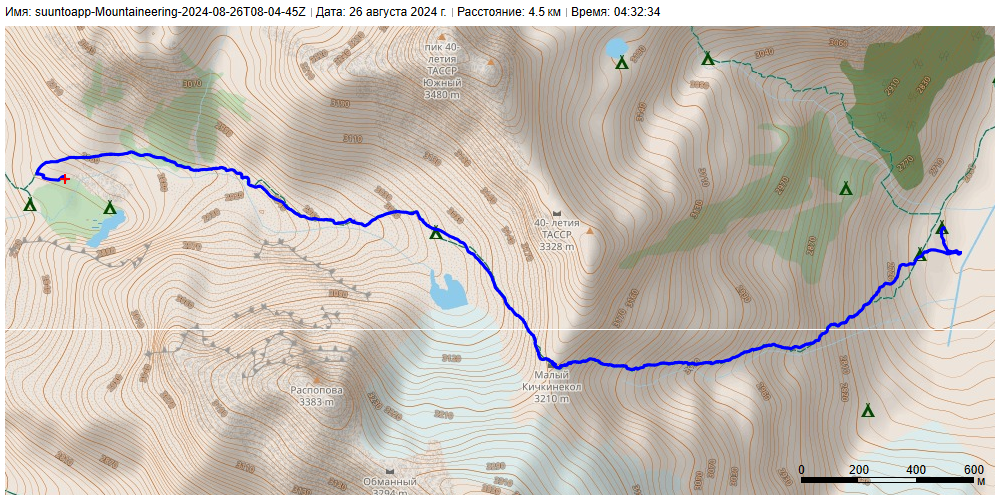
\includegraphics[angle=0, width=0.7\linewidth]{../pics/mini_maps/26}
	\label{fig:mini_26}
\end{figure}

Подъём в 08:00. Ночная гроза закончилась, небо было затянуто облаками, периодически проглядывало солнце. \alert{(Сушились?)} Вышли в 11:00, на тропу, траверсирующей травянистый склон. Эта тропа обходит водопад на западной оконечности поляны слева пхд. Встречаются туры, тропу видно хорошо. 
Постепенно травянистый склон переходит в морену.

\begin{figure}[h!]
	\centering
	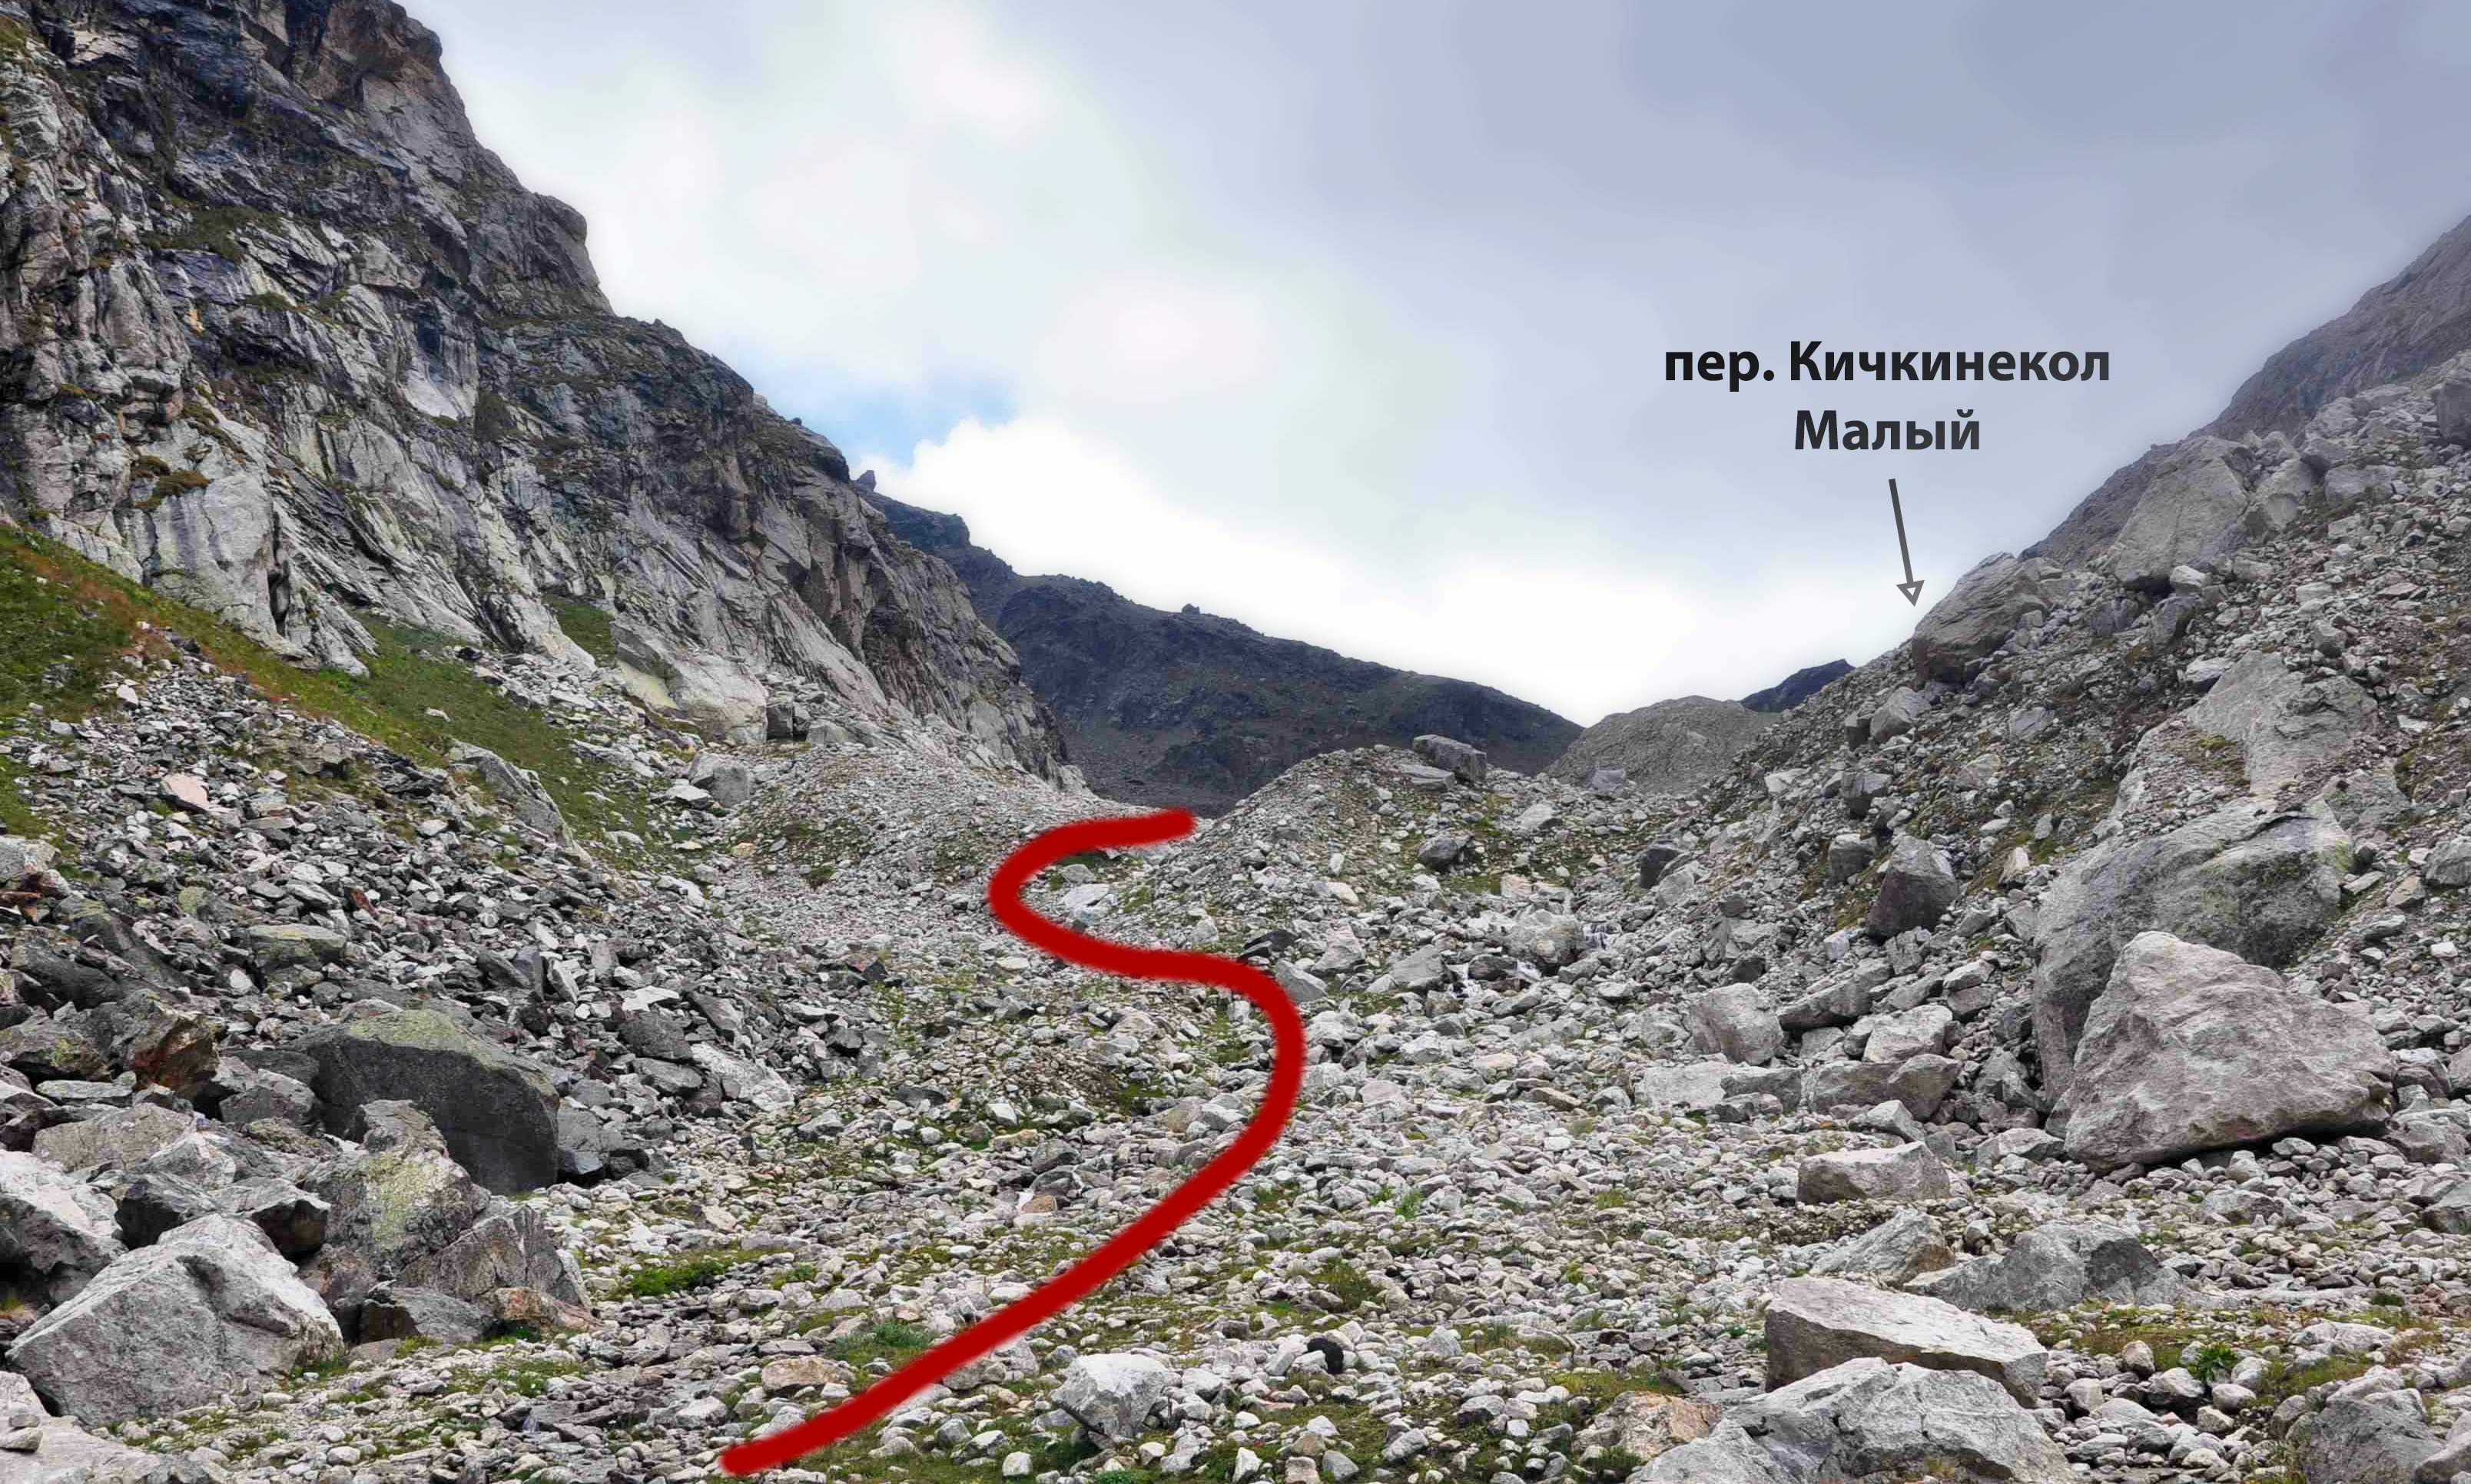
\includegraphics[width=0.7\linewidth]{../pics/DSC_0221.JPG}
	\caption{Путь подъёма на перевал}
	\label{fig:DSC_0221}
\end{figure}
 
За поворотом нам открылся вид на наш перевал и цирк соседнего перевала Обманный (рис.~\ref{fig:DSC_0226},\ref{fig:DSC_0227}).
 
\begin{figure}[h!]
	\centering
	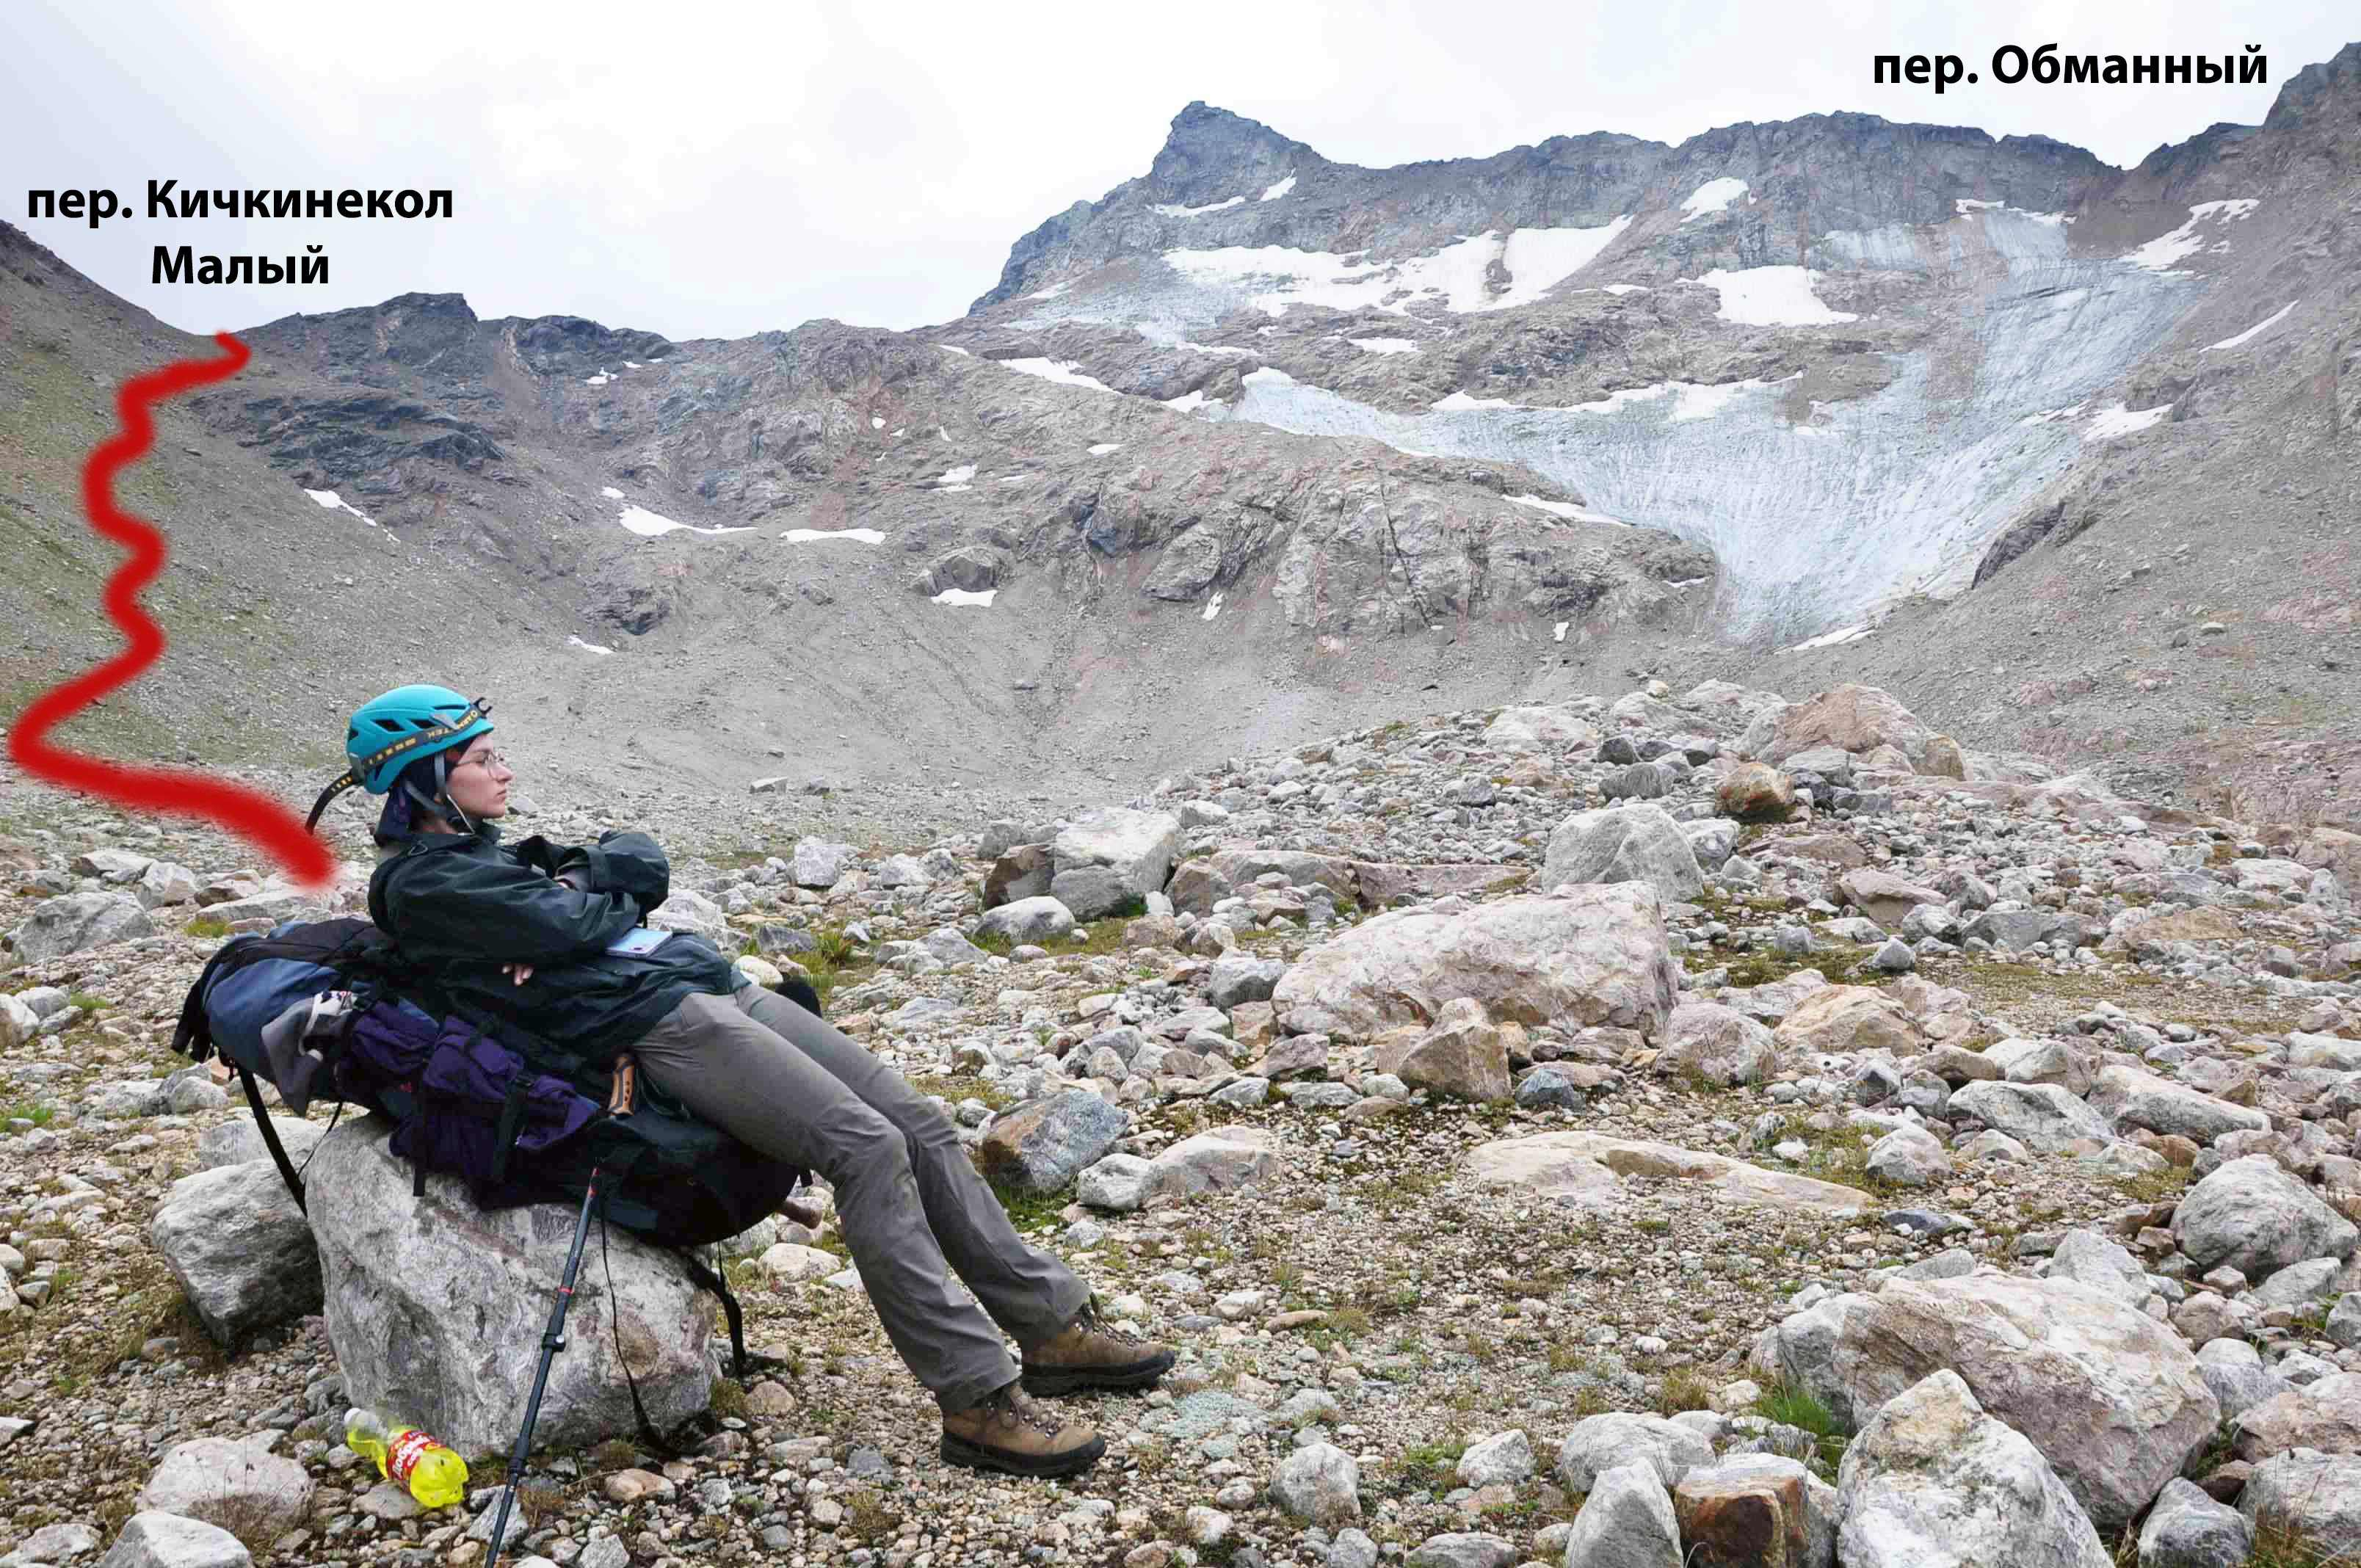
\includegraphics[width=0.7\linewidth]{../pics/DSC_0226}
	\caption{Маршрут движения группы}
	\label{fig:DSC_0226}
\end{figure}

Погода тем временем ухудшилась, начался небольшой дождь.


\begin{figure}[h!]
	\centering
	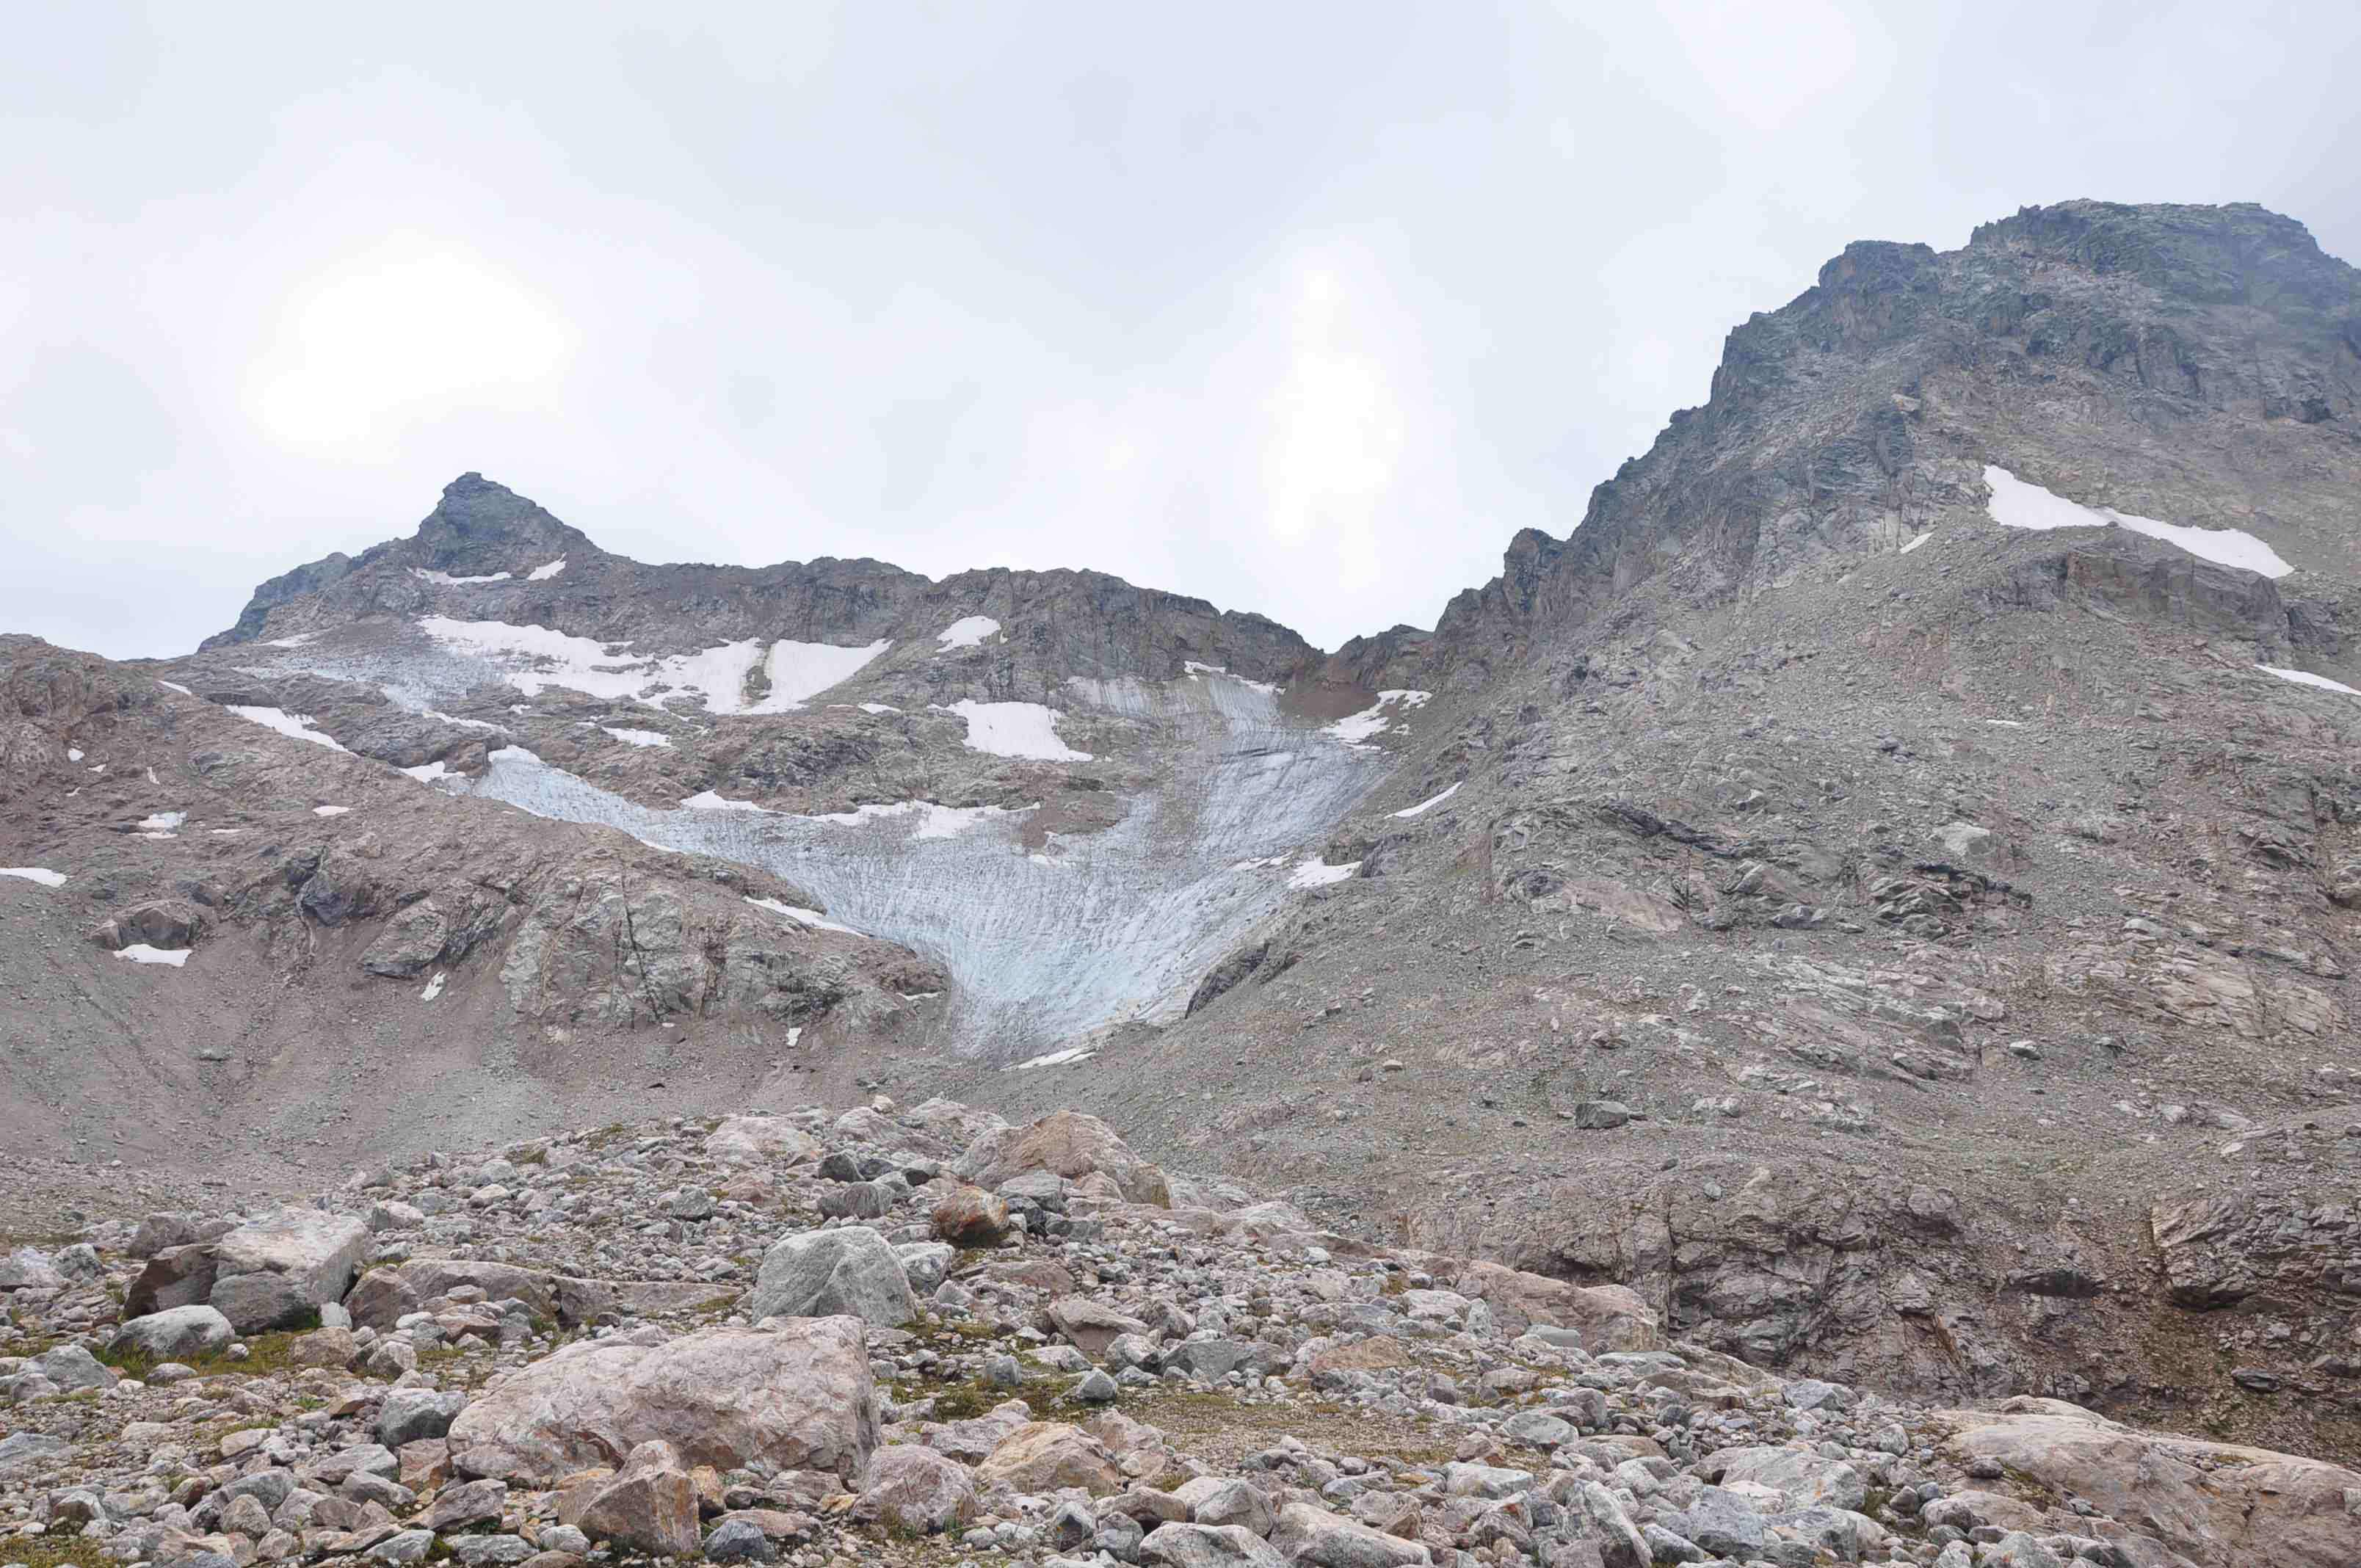
\includegraphics[width=0.7\linewidth]{../pics/DSC_0227.JPG}
	\caption{Цирк пер. Обманный справа пхд от пер. Кичкинекол Малый}
	\label{fig:DSC_0227}
\end{figure}


Подъём на перевал проходит по средней и мелкой осыпи; группа шла косыми траверсами с самостраховкой треккинговыми палками. Технической сложности подъём на Кичкинекол Малый не представляет.
В 13:15 вышли на седловину перевала (рис.~\ref{fig:DSC_0239}). Погода испортилась вконец, пошёл косой ливень с градом. Сняли перевальную записку т/к <<Крокус>> (г.~Краснодар) от 24.08.2024~г.; свою записку руководитель писал на каске участника, пока остальная группа укрывала их обоих полами дождевика-пончо. Кое-как запихнули в себя перевальный шоколад и в 13:22 начали спуск.


\begin{figure}[h!]
	\centering
	\begin{minipage}[h]{0.48\linewidth}
		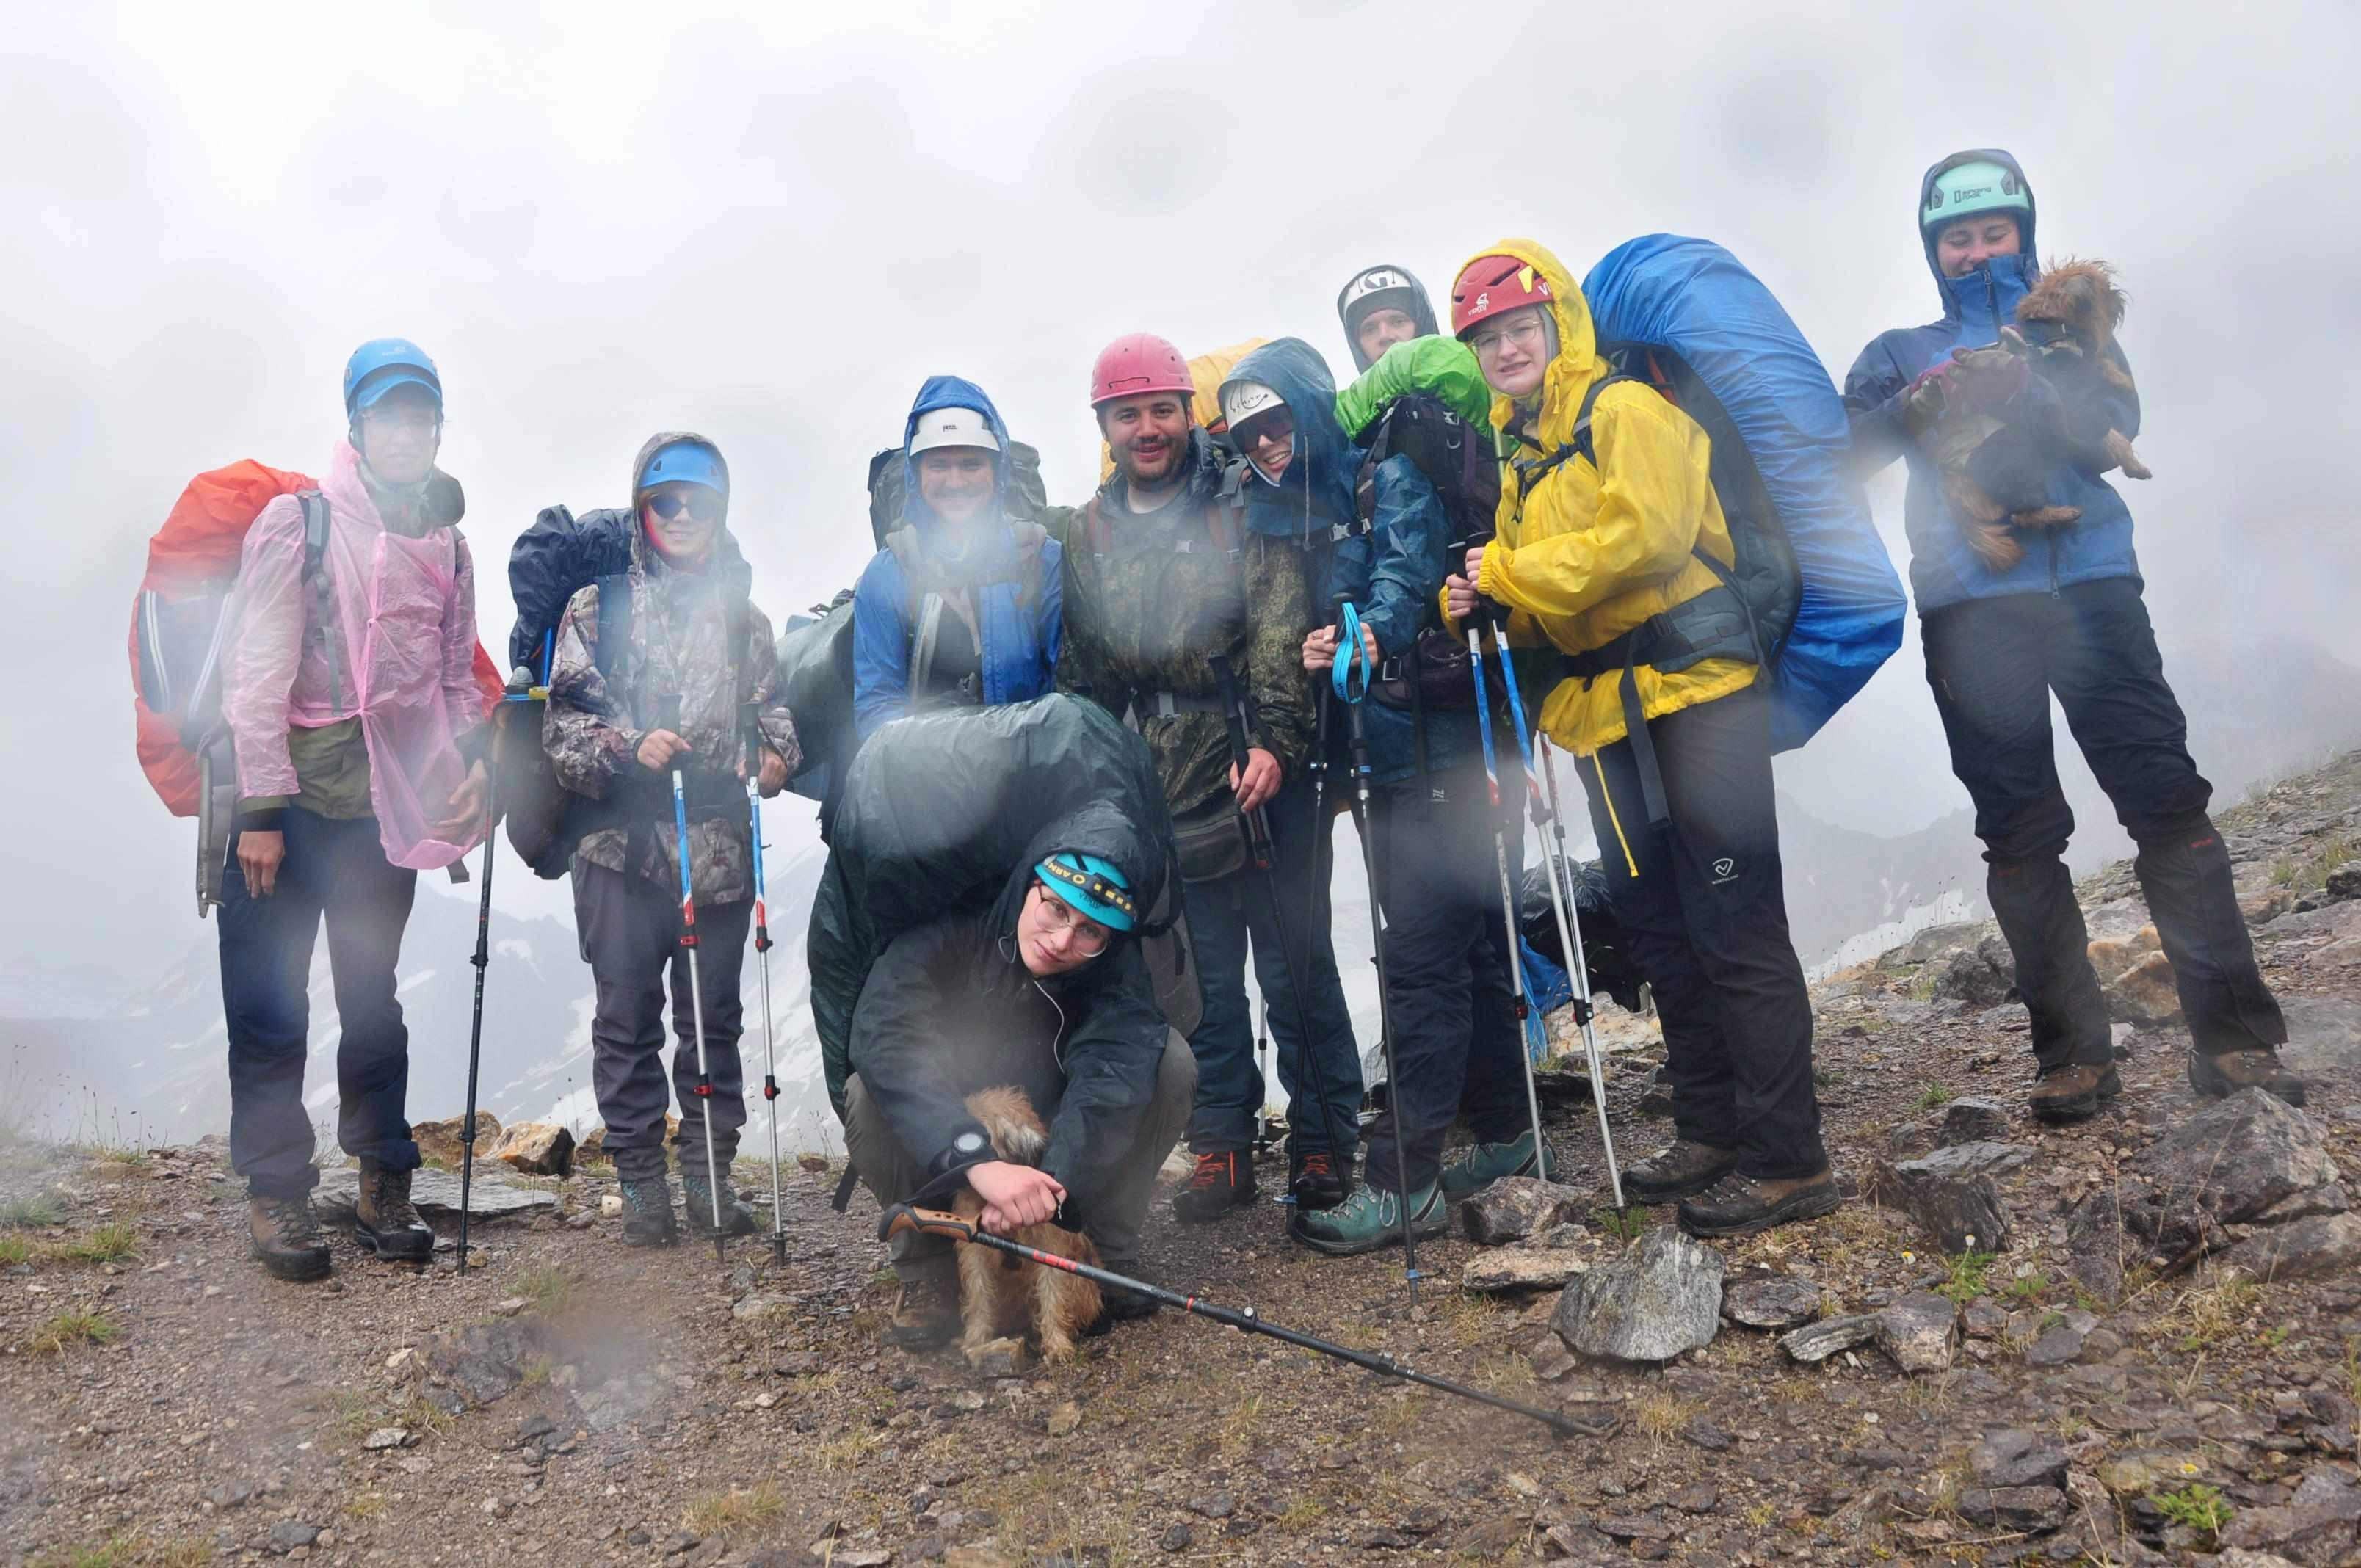
\includegraphics[width=0.99\linewidth]{../pics/DSC_0239.jpg}
	\end{minipage}
	\quad
	\begin{minipage}[h]{0.48\linewidth}
		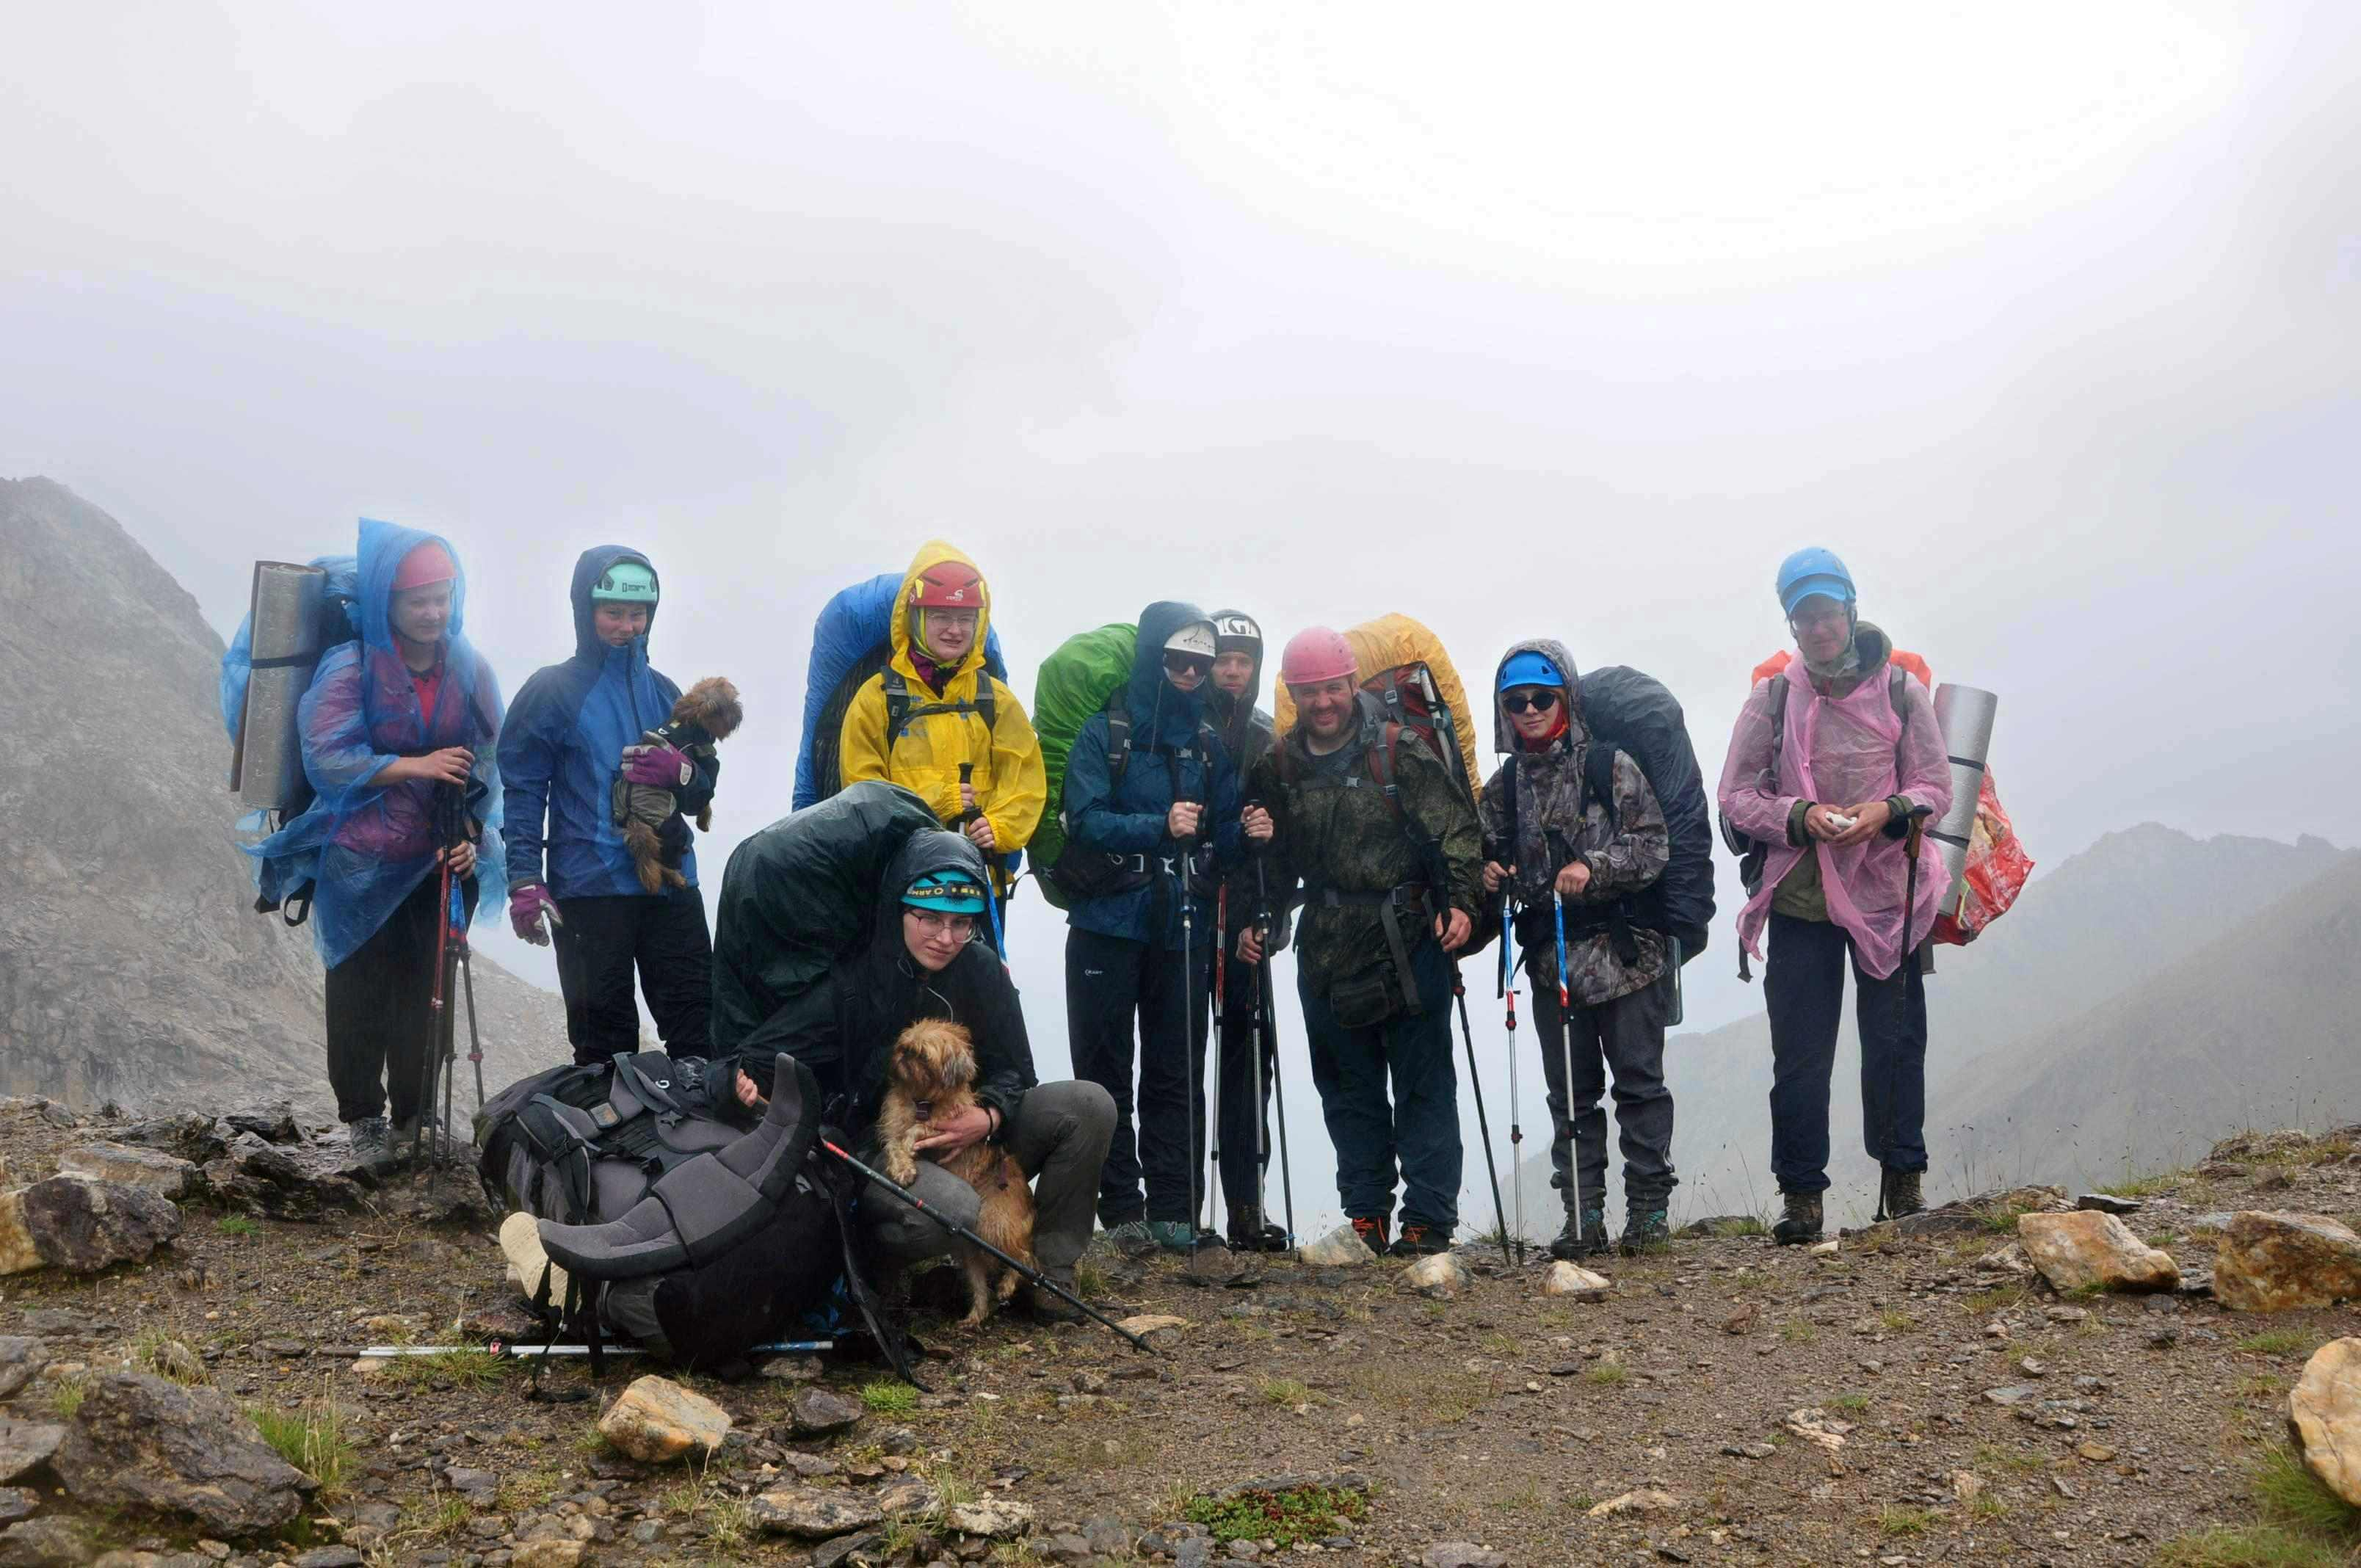
\includegraphics[width=0.99\linewidth]{../pics/DSC_0242.jpg}
	\end{minipage}
	\caption{Группа на пер. Кичкинекол Малый. Слева: вид в д.р. Чунгур-Джар, справа: вид в д.р. Таллычат}
	\label{fig:DSC_0239}
\end{figure}

Спуск с перевала идёт также по хорошо набитой тропе травянисто-осыпного склона; периодически встречаются туры. Справа от тропы нам открывался живописный вид на ГКХ, ледник Чунгур-Джар. Ливень тем временем превратился в мелкий дождь. В 15:00 спустились на урочище Аэродром в д.р Чунгур-Джар. Рельеф в этом месте представляет из себя бугристый конгломерат, поэтому поиск места для ночёвки представлял отдельную задачу. По воспоминаниям руководителя, их группа \cite{Korolyov2018} ночевала на правом берегу р. Чунгур-Джар, --- но это было при том, что группа отказалась от сквозного прохождения Перемётного, и могла позволить себе встать ниже по долине. То место ночёвки хорошо просматривалось, но для него требовалось перебродить реку, и, главное, довольно сильно спуститься, --- при том, что у нас ещё оставалась вероятность идти на следующий день на Перемётный. На левом же берегу были огороженные камнями места под палатки, которые, впрочем, не выглядели так чтобы очень уютно. Провели разведку с бродом: разведка показала, что на данном уровне на противоположном берегу палатку поставить точно нельзя, --- поэтому остановились на варианте с огороженными <<не очень уютными>> площадками. Дождь всё это время не прекращался, сопровождаясь сильным ветром.

Обед приготовили участники-<<волонтёры>>, которые чувствовали себя более-менее неплохо, --- остальные сушились и грелись в палатках. Координаты м.н.: N43.248385\degree,~E42.236151\degree.

\begin{table}[h!]
	\centering
	\begin{tabular}{|c|c|c|c|c|c|} 
		\hline 
		Этап & ЧХВ \\ 	
		\hline 
		От а/л <<Узункол>> до начала косого траверса  & 01:05 \\
		Подъём косым траверсом из д.р. Кичкинекол до нижних ночёвок  & 01:18 \\
		Подъём к Поляне Крокусов & 01:00\\ 
		Подъём на седловину перевала & 02:08\\ 
		Спуск с седловины до урочища <<Аєродром>> & 01:07 \\
		
		\hline
		\textsc{Полное время подъёма на перевал  }& 05:38\\
		\textsc{Полное время спуска с перевала }& 01:07 \\
		\textsc{Полное время прохождения перевала }& 06:45 \\
		\hline
	\end{tabular}
	\caption{Расклад времени, пер. Кичкинекол Малый}
\end{table}

\paragraph{Выводы и рекомендации:} \alert{(То же самое: черкни свою мыслю как-нибудь более развёрнуто, если можешь.)}

\clearpage